\documentclass[a4paper]{article}
\usepackage[utf8]{inputenc}
\usepackage[spanish, es-tabla, es-noshorthands]{babel}
\usepackage[table,xcdraw]{xcolor}
\usepackage[a4paper, footnotesep = 1cm, width=20cm, top=2.5cm, height=25cm, textwidth=18cm, textheight=25cm]{geometry}
%\geometry{showframe}

\usepackage{tikz}
\usepackage{amsmath}
\usepackage{amsfonts}
\usepackage{amssymb}
\usepackage{float}
\usepackage{graphicx}
\usepackage{caption}
\usepackage{subcaption}
\usepackage{multicol}
\usepackage{multirow}
\setlength{\doublerulesep}{\arrayrulewidth}
\usepackage{booktabs}

\usepackage{hyperref}
\hypersetup{
    colorlinks=true,
    linkcolor=blue,
    filecolor=magenta,      
    urlcolor=blue,
    citecolor=blue,    
}

\newcommand{\quotes}[1]{``#1''}
\usepackage{array}
\newcolumntype{C}[1]{>{\centering\let\newline\\\arraybackslash\hspace{0pt}}m{#1}}
\usepackage[american]{circuitikz}
\usetikzlibrary{calc}
\usepackage{fancyhdr}
\usepackage{units} 

\graphicspath{{../Ejercicio-1/}{../Ejercicio-2/}{../Ejercicio-3/}{../Ejercicio-4/}}

\pagestyle{fancy}
\fancyhf{}
\lhead{22.01 Teoría de Circuitos}
\rhead{Mechoulam, Lambertucci, Rodriguez Turco, Londero, Galdeman}
\rfoot{\centering \thepage}

\begin{document}

%%%%%%%%%%%%%%%%%%%%%%%%%
%		Caratula		%
%%%%%%%%%%%%%%%%%%%%%%%%%

\begin{titlepage}
\newcommand{\HRule}{\rule{\linewidth}{0.5mm}}
\center
\mbox{\textsc{\LARGE \bfseries {Instituto Tecnológico de Buenos Aires}}}\\[1.5cm]
\textsc{\Large 22.01 Teoría de Circuitos}\\[0.5cm]


\HRule \\[0.6cm]
{ \Huge \bfseries Trabajo práctico N$^{\circ}$5}\\[0.4cm] 
\HRule \\[1.5cm]


{\large

\emph{Grupo 3}\\
\vspace{3px}

\begin{tabular}{lr} 	
\textsc{Mechoulam}, Alan  &  58438\\
\textsc{Lambertucci}, Guido Enrique  & 58009 \\
\textsc{Rodriguez Turco}, Martín Sebastian  & 56629 \\
\textsc{Londero Bonaparte}, Tomás Guillermo  & 58150 \\
\textsc{Galdeman}, Agustín & 59827\\
\end{tabular}

\vspace{20px}

\emph{Profesores}\\
Jacoby, Daniel Andrés\\
Belaustegui Goitia, Carlos\\
Iribarren, Rodrigo Iñaki\\
\vspace{3px}
%\textsc{} \\	

\vspace{100px}

\begin{tabular}{ll}

Presentado: & */*/19\\

\end{tabular}

}

\vfill

\end{titlepage}


%%%%%%%%%%%%%%%%%%%%%
%		Indice		%
%%%%%%%%%%%%%%%%%%%%%

\tableofcontents
\newpage

%%%%%%%%%%%%%%%%%%%%%
%		Informe		%
%%%%%%%%%%%%%%%%%%%%%

\section{Introducción}
En este informe se presenta y se explica como se confeccionó el filtro final propuesto por la cátedra. Para este, se valió del uso de las aproximaciones y celdas estudiadas a lo largo de la materia, para luego poder satisfacer la plantilla establecida.

\section{Elaboración del filtro}
Dado que el filtro debe ser un rechaza banda, con aproximación de Chebycheff Inverso, se buscó que este cumpla con las siguientes restricciones:
\begin{table}[H]
\centering
\begin{tabular}{cc}
\hline
\textbf{Variable} & \textbf{Valor} \\
\hline
$f_p^-$ & 11.712 kHz   \\ 
$f_a^-$ & 13.802kHz    \\ 
$f_a^+$ & 16.301kHz    \\ 
$f_p^+$ & 19.211kHz    \\ 
$A_a$   & 45dB         \\ 
$A_p$   & 1dB          \\ 
k       & $\frac{1}{3}$ \\ 
\hline
\end{tabular}
\caption{Características del filtro realizado.}
\label{tabla:caracteristicas1}
\end{table}

Para ello, se decidió emplear celdas del tipo universal, más específicamente del tipo Fleischer-Tow. Es por ello que se analiza y se explica la selección de dicha celda a continuación. 

\subsection{Celda universal Fleischer-Tow (FT)}
En ocasiones es deseable poseer una señal de entrada que alimente varios nodos, obteniendo una única salida. A continuación se presenta la celda Fleischer-Tow, la cual se caracteriza por poder presentar una única transferencia que, dependiendo de los componentes seleccionados, puede ser un pasa bajos, pasa altos, pasa todo, de banda pasante y rechaza banda\footnote{R. Raut and M. N. S. Swamy, Modern Analog Filter Analysis and Design, 1st. ed. Weinheim: John Wiley and Sons, 2010.}, lo cual es una fuerte ventaja frente a los otros tipos de celdas universales, las cuales requieren más de tres operacionales para conseguir dichas salidas.

\begin{figure}[H]
\centering
	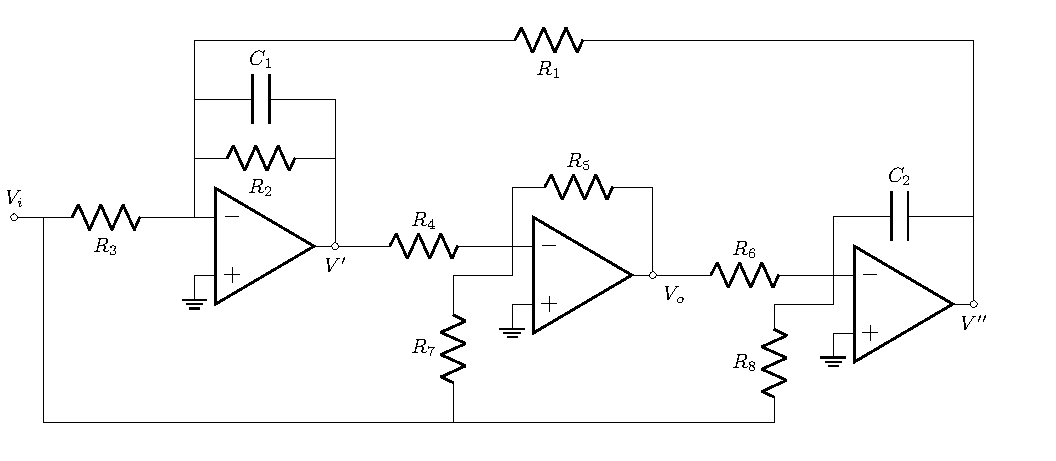
\includegraphics[width=0.9\textwidth]{Imagenes/FT.pdf}
	\caption{Circuito de la celda Universal Fleischer-Tow.}
\label{fig:FT}
\end{figure}

Se analiza el circuito presentado para poder obtener la transferencia de este. Para calcular la función mencionada de esta celda, se observa primero la siguiente configuración:
\begin{figure}[H]
\centering
\begin{circuitikz}
	\node [ocirc, label=left:$V_a$](va){};
	\draw (va.east) to[generic, l=$Z_1$] ++(3,0) node[op amp, anchor=-](A1){};
	\draw (va) ++(0.5,0) node[](v1aux1){};
	\draw (A1.+) node[ground](){};
	\draw (A1.out) node[](aux1){};	
	\draw (A1.-) -- ++(0,1) to[generic, l=$Z_3$] ++(2.25,0) -| (aux1.center);
	\draw (A1.out) -- ++(0.5,0) node[ocirc, label=below:$V_c$](){};
	\draw (A1.-) -- ($ (A1.-) !.7! (A1.+) $) to[generic, l=$Z_2$] ++(-3,0) node[ocirc, label=left:$V_b$](vb){};
\end{circuitikz}
\caption{Circuito genérico inversor.}
\label{fig:generic}
\end{figure}

Observando la Figura (\ref{fig:generic}), aplicando el teorema de superposición, se presenta una configuración inversora, por lo que se obtiene
\begin{equation}
	V_c = -\frac{V_a}{\frac{Z_1}{Z_3} + \frac{Z_1}{Z_3 A_o} + \frac{1}{A_o}} - \frac{V_b}{\frac{Z_2}{Z_3} + \frac{Z_2}{Z_3 A_o} + \frac{1}{A_o}}
	\label{equ:generic}
\end{equation}

Aplicando (\ref{equ:generic}) y considerando los tres operacionales de la Figura (\ref{fig:FT}) iguales, se obtiene el siguiente sistema de ecuaciones:
\begin{equation}
\begin{split}
	V' = - V_i A - V'' B \\
	V_o = - V' C - V_i D \\
	V'' = - V_o E - V_i F
\end{split}
\end{equation}
siendo las constantes empleadas las siguientes:
\begin{equation}
\begin{split}
	A^{-1} =& \ \frac{R_3}{R_2 // \frac{1}{sC_1}} + \frac{R_3}{\left( R_2 // \frac{1}{sC_1} \right) A_o} + \frac{1}{A_o} \\
	B^{-1} =& \ \frac{R_1}{R_2 // \frac{1}{sC_1}} + \frac{R_1}{\left( R_2 // \frac{1}{sC_1} \right) A_o} + \frac{1}{A_o} \\
	C^{-1} =& \ \frac{R_4}{R_5} + \frac{R_4}{R_5 A_o} + \frac{1}{A_o} \\
	D^{-1} =& \ \frac{R_7}{R_5} + \frac{R_7}{R_5 A_o} + \frac{1}{A_o} \\
	E^{-1} =& \ sC_2R_6 + \frac{sC_2R_6}{A_o} + \frac{1}{A_o} \\
	F^{-1} =& \ sC_2R_8 + \frac{sC_2R_8}{A_o} + \frac{1}{A_o}
\end{split}
\end{equation}

Operando algebraicamente, se obtiene que la transferencia de esta configuración es
\begin{equation}
	\frac{V_o}{V_i} = \frac{AC - BCF - D}{1 + BCE}
	\label{equ:transf-ft-r}
\end{equation}

Si se consideran ideales los operacionales, es decir, se toma $A_o \rightarrow \infty$, se obtiene que la forma de la transferencia final es
\begin{equation}
	\frac{V_o}{V_i} = - \frac{R_6}{R_8} \frac{s^{2} \frac{C_1 C_2 R_1 R_8 R_4}{R_7} + s \frac{C_2 R_1 R_8 R_4}{R_2} \left( \frac{1}{R_7} - \frac{R_2}{R_3 R_4} \right) + 1}{s^{2} \frac{C_1 C_2 R_6 R_1 R_4}{R_5} + s \frac{C_2 R_6 R_1 R_4}{R_2 R_5} + 1}
\label{equ:transf-ft-i}
\end{equation}

Es de interés obtener de esta los factores $\omega_o$ y $Q$ de los polos, siendo estos los presentados a continuación.
\begin{equation}
\begin{split}
	\omega_o = \sqrt{\frac{R_5}{R_6 R_1 R_4 C_1 C_2}} \\
	Q = R_2 \sqrt{\frac{C_1 R_5}{C_2 R_6 R_1 R_4}} 
\end{split}
\label{equ:woq-ft}
\end{equation}

Es así que se destaca la dependencia de $\omega_o$ y $Q$ de los capacitores, mientras que resultan ser independientes de $R_8$. Además,resulta de interes que la frecuencia del polo es independiente de la resistencia $R_2$, mientras que $Q$ no, lo que permite modificar la primer variable sin afectar a la segunda.

\subsection{Análisis de sensibilidades}
En la siguiente sección, se procede a calcular las sensibilidades de $H(s)$, $Q$ y $\omega_o$ con respecto de cada componente, definiéndose la sensibilidad de una función $y$ con respecto de $x$ de la forma:
\begin{equation*}
	S_{x}^{y} = \frac{\delta y}{\delta x} \frac{x}{y}
\end{equation*}

Primero, se presentan las sensibilidades de $H\left(s \right)$:
\begin{equation}
S_{R_2}^{H} = -{\frac {s \left[ s{C_2}\,{R_6}\,{R_1}\,{R_8}\,{R_7}+{
R_3}\, \left( -{R_6}\,{R_7}+{R_8}\,{R_5} \right) 
 \right] {C_2}\,{R_2}\,{R_1}\,{R_4}}{ \left[ {R_2}\,{
R_5}+{R_1}\, \left( {C_1}\,{R_2}\,s+1 \right) {R_4}\,s{
C_2}\,{R_6} \right]  \left[ s{R_1}\,{R_8}\, \left( {C_1
}\,{R_2}\,{R_3}\,{R_4}\,s-{R_2}\,{R_7}+{R_3}\,{R_4} \right) {C_2}+{R_2}\,{R_3}\,{R_7} \right] }}
\end{equation}

\begin{equation}
S_{R_6}^{H} =	{\frac {{R_2}\,{R_5}}{{R_1}\, \left( {C_1}\,{R_2}\,s+1
 \right) {R_4}\,s{C_2}\,{R_6}} \left[ {\frac {{R_2}\,{R_5}}{{R_1}\, \left( {C_1}\,{R_2}\,s+1 \right) {R_4}\,s{
C_2}\,{R_6}}}+1 \right] ^{-1}}
\end{equation}

\begin{equation}
S_{R_1}^{H} = {\frac { \left\lbrace  \left[ s{C_1}\,{R_3}\, \left( -{R_6}\,{R_7}+{R_8}\,{R_5} \right) {R_4}-{R_5}\,{R_8}\,{R_7}
 \right] {R_2}+{R_4}\,{R_3}\, \left( -{R_6}\,{R_7}+{
R_8}\,{R_5} \right)  \right\rbrace s{C_2}\,{R_2}\,{R_1}}{
 \left[  \left( {C_1}\,{C_2}\,{R_6}\,{R_1}\,{R_4}\,{s}^
{2}+{R_5} \right) {R_2}+{R_1}\,{R_4}\,s{C_2}\,{R_6}
 \right]  \left\lbrace  \left[ {s}^{2}{R_4}\,{C_1}\,{C_2}\,{R_1}
\,{R_3}\,{R_8}-{R_7}\, \left( {C_2}\,{R_1}\,{R_8}\,s
-{R_3} \right)  \right] {R_2}+{R_1}\,{R_4}\,s{C_2}\,{
R_8}\,{R_3} \right\rbrace }}
\end{equation}

\begin{equation}
S_{R_3}^{H} = -{\frac {{R_2}\,{R_5}}{{R_3}\, \left( {C_1}\,{R_2}\,s+1
 \right) {R_4}} \left[ -{\frac {{R_2}\,{R_5}}{{R_1}\,
 \left( {C_1}\,{R_2}\,s+1 \right) {R_4}\,s{C_2}\,{R_8}}
}+{\frac {{R_2}\,{R_5}}{{R_3}\, \left( {C_1}\,{R_2}\,s+
1 \right) {R_4}}}-{\frac {{R_5}}{{R_7}}} \right] ^{-1}}
\end{equation}

\begin{equation}
s_{R_8}^{H} ={\frac {{R_2}\,{R_5}}{{R_1}\, \left( {C_1}\,{R_2}\,s+1
 \right) {R_4}\,s{C_2}\,{R_8}} \left[ -{\frac {{R_2}\,{
R_5}}{{R_1}\, \left( {C_1}\,{R_2}\,s+1 \right) {R_4}\,s
{C_2}\,{R_8}}}+{\frac {{R_2}\,{R_5}}{{R_3}\, \left( {
C_1}\,{R_2}\,s+1 \right) {R_4}}}-{\frac {{R_5}}{{R_7}}}
 \right] ^{-1}}
\end{equation}

\begin{equation}
S_{R_7}^{H} ={\frac {{R_5}}{{R_7}} \left[ -{\frac {{R_2}\,{R_5}}{{R_1}\, \left( {C_1}\,{R_2}\,s+1 \right) {R_4}\,s{C_2}\,{
R_8}}}+{\frac {{R_2}\,{R_5}}{{R_3}\, \left( {C_1}\,{
R_2}\,s+1 \right) {R_4}}}-{\frac {{R_5}}{{R_7}}} \right]^{-1}}
\end{equation}

\begin{equation}
S_{R_4}^{H} = {\frac { s \left( {C_1}\,{R_2}\,s+1 \right) \left[ s{C_2}\,{
R_6}\,{R_1}\,{R_8}\,{R_7}+{R_3}\, \left( -{R_6}\,{
R_7}+{R_8}\,{R_5} \right)  \right] {C_2}\,{R_2}\,{R_1}\,{R_4}}{ \left( {C_1}\,{C_2}\,{R_2}\,{R_6}\,{R_1
}\,{R_4}\,{s}^{2}+{R_1}\,{R_4}\,s{C_2}\,{R_{6}}+{R_2}
\,{R_5} \right)  \left[ {s}^{2}{R_4}\,{C_1}\,{C_2}\,{R_2}\,{R_1}\,{R_3}\,{R_8}+{C_2}\,{R_1}\,{R_8}\,
 \left( -{R_2}\,{R_7}+{R_3}\,{R_4} \right) s+{R_2}\,{
R_3}\,{R_7} \right] }}
\end{equation}

\begin{equation}
S_{R_5}^{H} = {\frac {{R_1}\, \left( {C_1}\,{R_2}\,s+1 \right) {R_4}\,s{
C_2}\,{R_6}}{{R_2}\,{R_5}+{R_1}\, \left( {C_1}\,{
R_2}\,s+1 \right) {R_4}\,s{C_2}\,{R_6}}}
\end{equation}

\begin{equation}
S_{C_1}^{H} = {\frac {{C_1}\,{s}^{2} \left[ s{C_2}\,{R_6}\,{R_1}\,{R_8}\,{R_7}+{R_3}\, \left( -{R_6}\,{R_7}+{R_8}\,{R_5}
 \right)  \right] {C_2}\,{{R_2}}^{2}{R_1}\,{R_4}}{ \left[ 
{R_2}\,{R_5}+{R_1}\, \left( {C_1}\,{R_2}\,s+1 \right) {
R_4}\,s{C_2}\,{R_6} \right]  \left[ s{R_1}\,{R_8}\,
 \left( {C_1}\,{R_2}\,{R_3}\,{R_4}\,s-{R_2}\,{R_7}+{
R_3}\,{R_4} \right) {C_2}+{R_2}\,{R_3}\,{R_7}
 \right] }}
\end{equation}

\begin{equation}
S_{C_2}^{H} = {\frac { \left\lbrace  \left[ s{C_1}\,{R_3}\, \left( -{R_6}\,{R_7}+{R_8}\,{R_5} \right) {R_4}-{R_5}\,{R_8}\,{R_7}
 \right] {R_2}+{R_4}\,{R_3}\, \left( -{R_6}\,{R_7}+{
R_8}\,{R_5} \right)  \right\rbrace s{C_2}\,{R_2}\,{R_1}}{
 \left[  \left( {C_1}\,{C_2}\,{R_6}\,{R_1}\,{R_4}\,{s}^
{2}+{R_5} \right) {R_2}+{R_1}\,{R_4}\,s{C_2}\,{R_6}
 \right]  \left\lbrace  \left[ {s}^{2}{R_4}\,{C_1}\,{C_2}\,{R_1}
\,{R_3}\,{R_8}-{R_7}\, \left( {C_2}\,{R_1}\,{R_8}\,s
-{R_3} \right)  \right] {R_2}+{R_1}\,{R_4}\,s{C_2}\,{
R_8}\,{R_3} \right\rbrace }}
\end{equation}

Luego, dado que la sensibilidades de $\omega_o$ y $Q$ resultan constantes, independientemente del componente del cual se las calcula, se presenta dichos valores de interés en la siguiente tabla.
\begin{table}[H]
\centering
\begin{tabular}{ccccccccccc}
\hline
 & $\mathbf{R_2}$ & $\mathbf{R_6}$ & $\mathbf{R_1}$ & $\mathbf{R_3}$ & $\mathbf{R_8}$ & $\mathbf{R_7}$ & $\mathbf{R_4}$ & $\mathbf{R_5}$ & $\mathbf{C_1}$ & $\mathbf{C_2}$ \\
\hline
$\omega_o$ & 0 & -0.5 & -0.5 & 0 & 0 & 0 & -0.5 & 0.5 & -0.5 & -0.5 \\
$Q$ & 1 & -0.5 & -0.5 & 0 & 0 & 0 & -0.5 & 0.5 & 0.5 & -0.5	\\
\hline
\end{tabular}
\caption{Sensibilidades de $\omega_o$ y $Q$ con respecto de cada componente}
\end{table}

\newpage
\section{Selección de componentes}
A continuación se presentan los componentes seleccionados para cada etapa.
\begin{multicols}{2}
\begin{table}[H]
\centering
\begin{tabular}{ccc}
\hline
\multicolumn{1}{c}{Componente} & \multicolumn{1}{c}{Valor} & Composición \\ \hline
$R_1$                           & 33.68 $k\Omega$                     & 680 $k\Omega$ + 33 $k\Omega$     \\
$R_2$                           & 334.28 $k\Omega$                    & 3.9 $k\Omega$ + 330 $k\Omega$   \\
$R_3$                           & 47 $k\Omega$                        & 47 $k\Omega$         \\
$R_4$                           & 334.28 $k\Omega$                    & 3.9 $k\Omega$ + 330 $k\Omega$   \\
$R_5$                           & 47 $k\Omega$                        & 47 $k\Omega$         \\
$R_6$                           & 49.7 $k\Omega$                        & 2.7 $k\Omega$ + 47 $k\Omega$         \\
$R_7$                           & 47 $k\Omega$                        & 47 $k\Omega$         \\
$R_8$                           & 50 $k\Omega$                        & 47 $k\Omega$+3 $k\Omega$         \\
$C_1$                           & 95 $pf$                        & 68 $pf$//27 $pf$     \\
$C_2$                           & 95 $pf$                        & 68 $pf$ //27 $pf$    \\
\hline
\end{tabular}
\caption{Componentes seleccionados de la primer etapa.}
\end{table}

\begin{table}[H]
\centering
\begin{tabular}{ccc}
\hline
\multicolumn{1}{c}{Componente} & \multicolumn{1}{c}{Valor} & Composición  \\ \hline
$R_1$                           & 27.03                      & 27+27 $k\Omega$      \\
$R_2$                           & 371.57 $k\Omega$                    & 680 $k\Omega$ // 820 $k\Omega$ \\
$R_3$                           & 47 $k\Omega$                        & 47 $k\Omega$          \\
$R_4$                           & 371.57 $k\Omega$                    & 680 $k\Omega$ // 820 $k\Omega$   \\
$R_5$                           & 52.5 $k\Omega$                      & 56 $k\Omega$ // 820 $k\Omega$    \\
$R_6$                           & 49.77 $k\Omega$                     & 2.7 $k\Omega$ + 47 $k\Omega$     \\
$R_7$                           & 47 $k\Omega$                        & 47 $k\Omega$          \\
$R_8$                           & 47.5 $k\Omega$                        & 47 $k\Omega$ + 500 $k\Omega$          \\
$C_1$                           & 100 $pf$                       & 100 $pf$         \\
$C_2$ 							& 100 $pf$                       & 100 $pf$          \\
\hline
\end{tabular}
\caption{Componentes seleccionados de la segunda etapa.}
\end{table}
\end{multicols}

\begin{multicols}{2}
\begin{table}[H]
\centering
\begin{tabular}{ccc}
\hline
\multicolumn{1}{c}{Componente} & \multicolumn{1}{c}{Valor} & Composición \\ \hline
$R_1$                           & 27.13                      & 120+27 $k\Omega$     \\
$R_2$                           & 465.31 $k\Omega$                    & 680 $k\Omega$ // 1.5 $M\Omega$  \\
$R_3$                           & 47 $k\Omega$                        & 47 $k\Omega$         \\
$R_4$                           & 465.31 $k\Omega$                    & 680 $k\Omega$ // 1.5 $M\Omega$  \\
$R_5$                           & 42.08 $k\Omega$                     & 15 $k\Omega$ + 27 $k\Omega$     \\
$R_6$                           & 49.77 $k\Omega$                     & 2.7 $k\Omega$ + 47 $k\Omega$    \\
$R_7$                           & 47 $k\Omega$                        & 47 $k\Omega$         \\
$R_8$                           & 48 $k\Omega$                        & 47 $k\Omega$ + 1 $k\Omega$         \\
$C_1$                           & 100 $pf$                       & 100 $pf$        \\
$C_2$                           & 100 $pf$                       & 100 $pf$        \\
\hline
\end{tabular}
\caption{Componentes seleccionados de la tercer etapa.}
\end{table}

\begin{table}[H]
\centering
\begin{tabular}{ccc}
\hline
\multicolumn{1}{c}{Componente} & \multicolumn{1}{c}{Valor} & Composición \\ \hline
$R_1$                           & 10.29 $k\Omega$                     & 4.7 $k\Omega$ + 5.6 $k\Omega$   \\
$R_2$                           & 1.32 $M\Omega$                      & 120 $k\Omega$ + 1.2 $M\Omega$   \\
$R_3$                           & 47 $k\Omega$                        & 47 $k\Omega$         \\
$R_4$                           & 1.32 $M\Omega$                      & 120 $k\Omega$ + 1.2 $M\Omega$   \\
$R_5$                           & 39.44 $k\Omega$                     & 470 $k\Omega$ + 39 $k\Omega$     \\
$R_6$                           & 49.77 $k\Omega$                     & 2.7 $k\Omega$ + 47 $k\Omega$    \\
$R_7$                           & 47 $k\Omega$                        & 47 $k\Omega$         \\
$R_8$                           & 48 $k\Omega$                        & 47 $k\Omega$ + 1 $k\Omega$         \\
$C_1$                           & 92 $pf$                        & 10 $pf$ // 82 $pf$  \\
$C_2$                           & 92 $pf$                        & 10 $pf$ // 82 $pf$  \\
\hline
\end{tabular}
\caption{Componentes seleccionados de la cuarta etapa.}
\end{table}
\end{multicols}

\begin{multicols}{2}
\begin{table}[H]
\centering
\begin{tabular}{ccc}
\hline
\multicolumn{1}{c}{Componente} & \multicolumn{1}{c}{Valor} & Composición \\ \hline
$R_1$                           & 10.19 $k\Omega$                     & 12 $k\Omega$ // 68 $k\Omega$    \\
$R_2$                           & 918.2 $k\Omega$                     & 100 $k\Omega$ + 820 $k\Omega$   \\
$R_3$                           & 47 $k\Omega$                        & 47 $k\Omega$         \\
$R_4$                           & 918.2 $k\Omega$                     & 100 $k\Omega$ + 820 $k\Omega$   \\
$R_5$                           & 56 $k\Omega$                        & 56 $k\Omega$         \\
$R_6$                           & 49.77 $k\Omega$                     & 2.7 $k\Omega$ + 47 $k\Omega$    \\
$R_7$                           & 45 $k\Omega$                        & 43 $k\Omega$ + 2 $k\Omega$         \\
$R_8$                           & 55 $k\Omega$                        & 12 $k\Omega$ + 43 $k\Omega$         \\
$C_1$                           & 88 $pf$                      & 82 $pf$ // 5.6 $pf$    \\
$C_2$                           & 88 $pf$                      & 82 $pf$ // 5.6 $pf$   \\
\hline
\end{tabular}
\caption{Componentes seleccionados de la quinta etapa.}
\end{table}

\begin{table}[H]
\centering
\begin{tabular}{ccc}
\hline
\multicolumn{1}{c}{Componente} & \multicolumn{1}{c}{Valor} & Composición \\ \hline
$R_1$                           & 27.13 $k\Omega$                      & 120 $k\Omega$ + 27 $k\Omega$     \\
$R_2$                           & 465.31 $k\Omega$                    & 680 $k\Omega$ // 1.5 $M\Omega$  \\
$R_3$                           & 47 $k\Omega$                        & 47 $k\Omega$         \\
$R_4$                           & 465.31 $k\Omega$                    & 680 $k\Omega$ // 1.5 $M\Omega$  \\
$R_5$                           & 42.08 $k\Omega$                     & 15 $k\Omega$ + 27 $k\Omega$     \\
$R_6$                           & 49.77 $k\Omega$                     & 2.7 $k\Omega$ + 47 $k\Omega$    \\
$R_7$                           & 46 $k\Omega$                        & 43 $k\Omega$ + 3 $k\Omega$         \\
$R_8$                           & 53 $k\Omega$                        & 51 $k\Omega$ + 2 $k\Omega$         \\
$C_1$                           & 70 $pf$                       & 68 $pf$        \\
$C_2$                           & 70 $pf$                       & 68 $pf$  \\
\hline
\end{tabular}
\caption{Componentes seleccionados de la sexta etapa.}
\end{table}
\end{multicols}

\subsection{Confección del circuito}
Al momento de elaborar el sistema en PCB se tuvieron ciertas consideraciones. Es común que, dado el factor $Q$ del circuito, un filtro del tipo notch introduzca un sobrepico en una zona previa o posterior a la banda rechazada. Es por ello que se decidió introducir presets que permitan el ajuste adecuado del sistema. Se introdujeron dichas resistencias variables en las impedancias $R_2$ de las etapas 1 y 5 y $R_7$ de las etapas 5 y 6. $R_2$ permite modificar la ganancia de banda pasante y el factor $Q$ de los polos, mientras que $R_7$ el $\omega_o$ de los ceros y la ganancia de banda pasante. De esta forma se pudo configurar el sistema para que se presente el menor sobre pico en banda pasante y garantizar la atenuación máxima de $1 \ dB$ en dicha etapa.

De esta forma, se confeccionó el siguiente PCB.
\begin{figure}[H]
\centering
	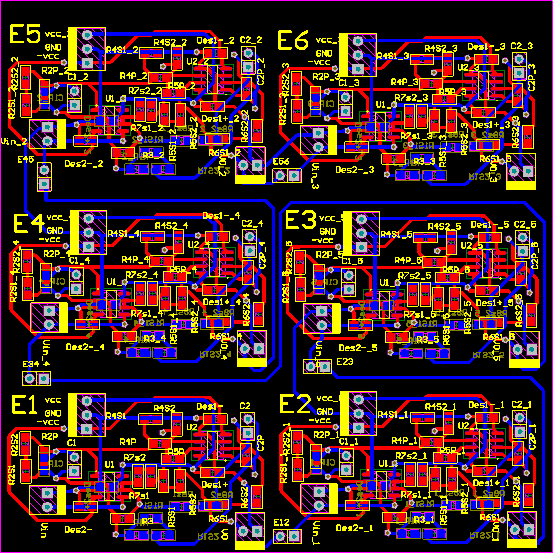
\includegraphics[width=0.5\textwidth]{Imagenes/PCB.png}
	\caption{PCB elaborado.}
\label{fig:pcb}
\end{figure}

Se decidió además confeccionar un diagrama de polos y ceros del circuito completo. De esta forma, se sabe que si los diagramas de Bode medidos y teóricos se corresponden, entonces los polos y ceros también lo harán.
\begin{figure}[H]
\centering
	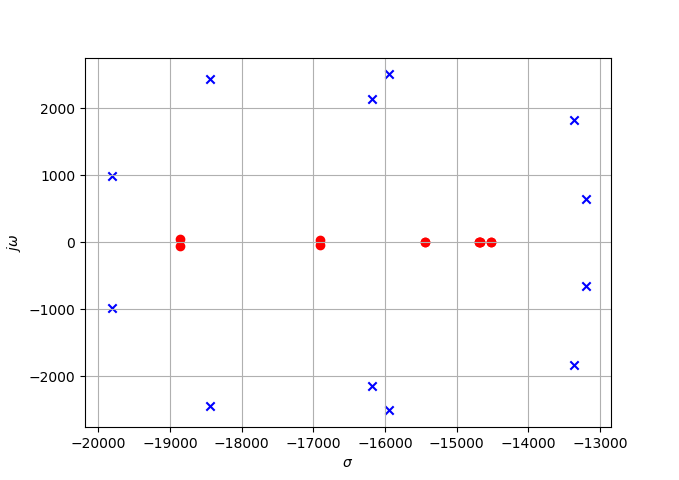
\includegraphics[width=0.5\textwidth]{Imagenes/PolosyCeros.png}
	\caption{Diagrama de polos y ceros del circuito total.}
\label{fig:pyc}
\end{figure}

Se remarca que, recorriendo de derecha a izquierda, los tres primeros ceros son ceros dobles, los cuales se encuentran superpuestos, dificultando su visualización.

Luego, al momento de confeccionar la placa, se decidió colocar terminales junto con jumpers de forma que sea posible desconectar las etapas entre sí, asilandolas para poder medirlas por separado. De esta forma, se procedió a medir cada etapa y contrastar dicho resultado con las curvas teóricas y simuladas, estas últimas obtenidas mediante el software LTSpice.
\begin{figure}[H]
\centering
\begin{subfigure}{.49\textwidth}
\centering
	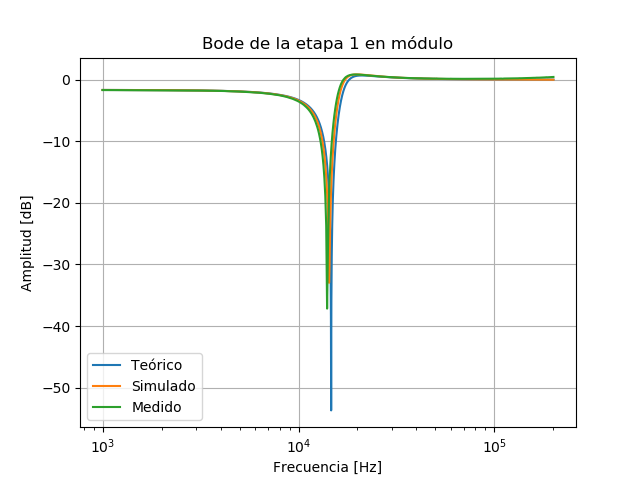
\includegraphics[width=\textwidth]{Imagenes/Mod-1.png}
	\caption{Ganancia de tensión de la primer etápa en módulo.}
	\label{fig:mod1}
\end{subfigure}
\centering
\begin{subfigure}{.49\textwidth}
\centering
	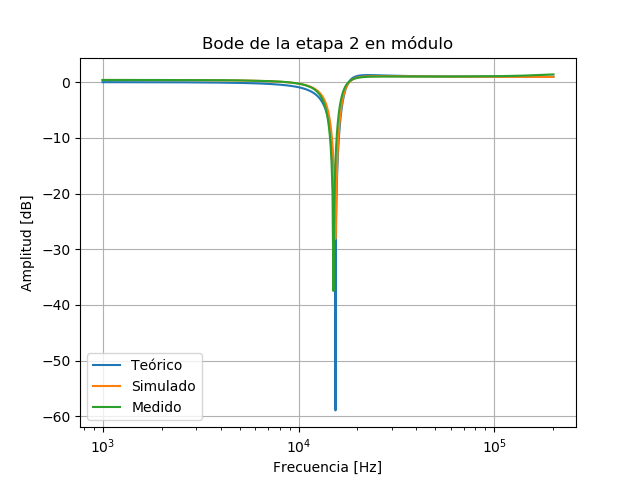
\includegraphics[width=\textwidth]{Imagenes/Mod-2.png}
	\caption{Diagrama de Bode de la segunda etápa en módulo.}
	\label{fig:mod2}
\end{subfigure}
\centering
\begin{subfigure}{.49\textwidth}
\centering
	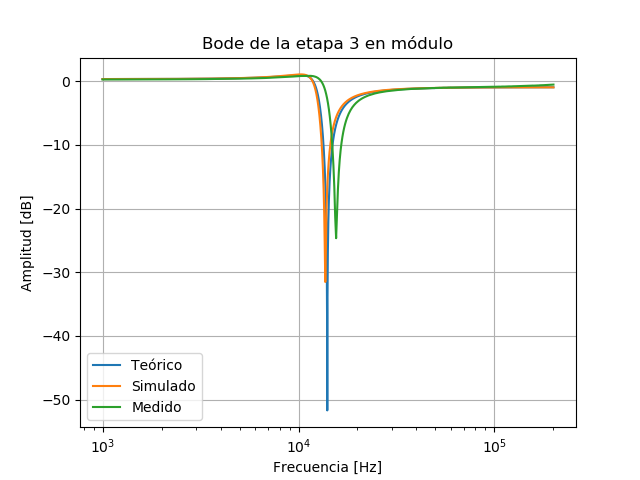
\includegraphics[width=\textwidth]{Imagenes/Mod-3.png}
	\caption{Diagrama de Bode de la tercer etápa en módulo.}
	\label{fig:mod3}
\end{subfigure}
\centering
\begin{subfigure}{.49\textwidth}
\centering
	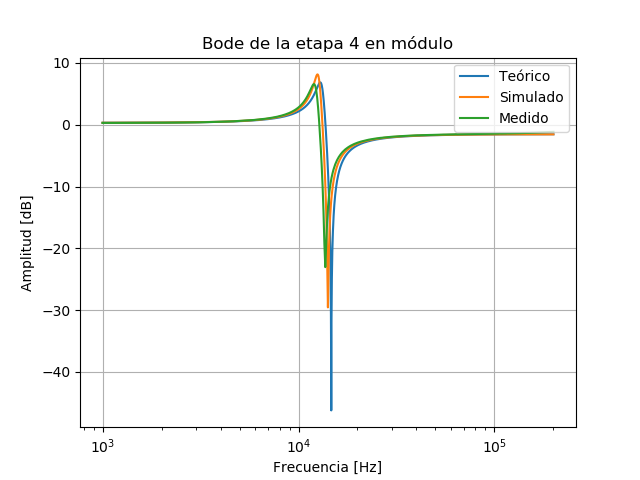
\includegraphics[width=\textwidth]{Imagenes/Mod-4.png}
	\caption{Diagrama de Bode de la cuarta etápa en módulo.}
	\label{fig:mod4}
\end{subfigure}
\centering
\begin{subfigure}{.49\textwidth}
\centering
	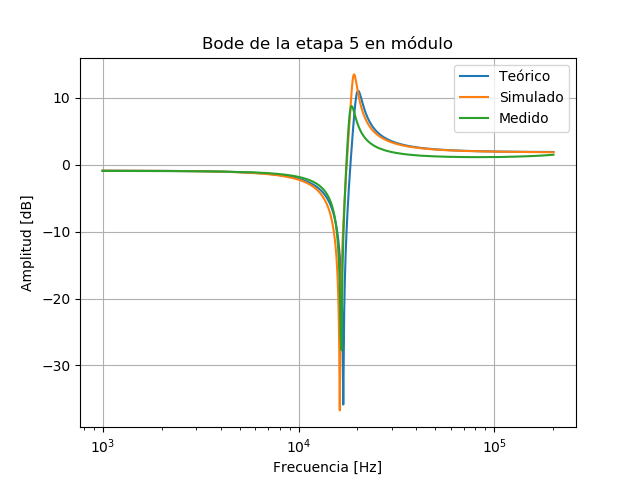
\includegraphics[width=\textwidth]{Imagenes/Mod-5.png}
	\caption{Diagrama de Bode de la quinta etápa en módulo.}
	\label{fig:mod5}
\end{subfigure}
\centering
\begin{subfigure}{.49\textwidth}
\centering
	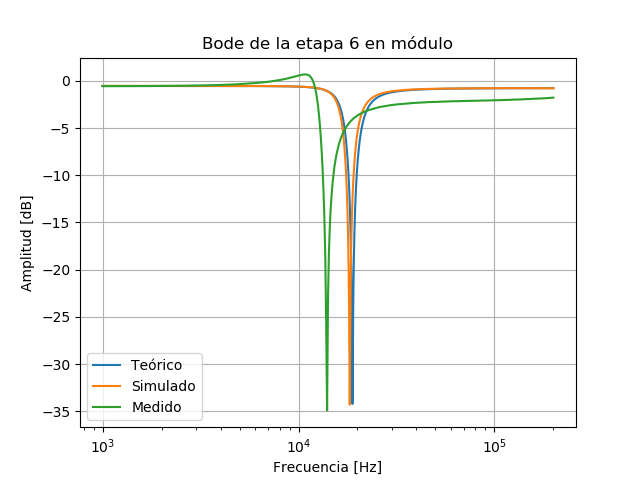
\includegraphics[width=\textwidth]{Imagenes/Mod-6.png}
	\caption{Diagrama de Bode de la sexta etápa en módulo.}
	\label{fig:mod6}
\end{subfigure}
\caption{Comparación de los Bodes de las etapas en módulo.}
\label{fig:bode-mag}
\end{figure}

Se atribuyen las pequeñas discrepancias entre las curvas a los presets puestos, ya que no se pudo determinar su valor con exactitud.

\begin{figure}[H]
\centering
\begin{subfigure}{.49\textwidth}
\centering
	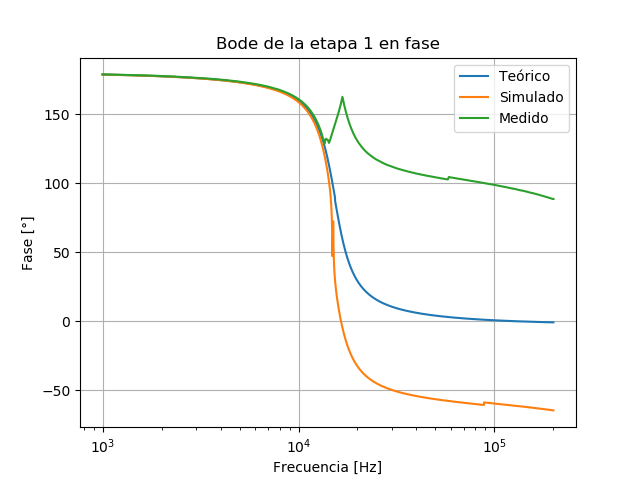
\includegraphics[width=\textwidth]{Imagenes/Pha-1.png}
	\caption{Diagrama de Bode de la primer etápa en fase.}
	\label{fig:pha1}
\end{subfigure}
\centering
\begin{subfigure}{.49\textwidth}
\centering
	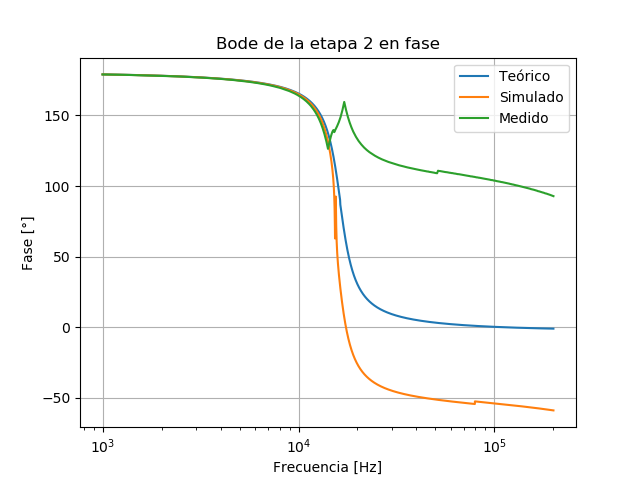
\includegraphics[width=\textwidth]{Imagenes/Pha-2.png}
	\caption{Diagrama de Bode de la segunda etápa en fase.}
	\label{fig:pha2}
\end{subfigure}
\centering
\begin{subfigure}{.49\textwidth}
\centering
	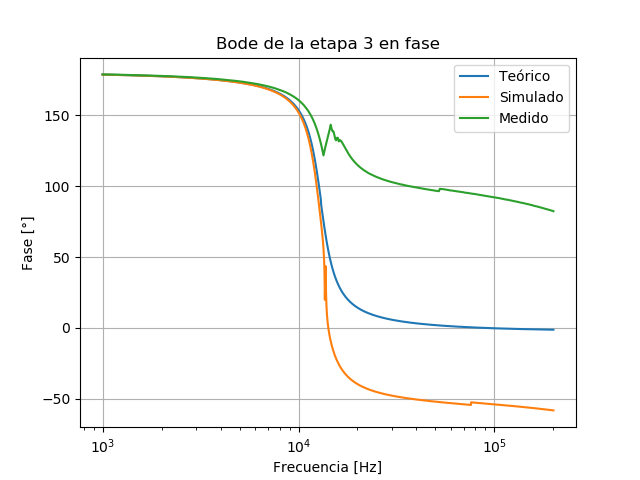
\includegraphics[width=\textwidth]{Imagenes/Pha-3.png}
	\caption{Diagrama de Bode de la tercer etápa en fase.}
	\label{fig:pha3}
\end{subfigure}
\centering
\begin{subfigure}{.49\textwidth}
\centering
	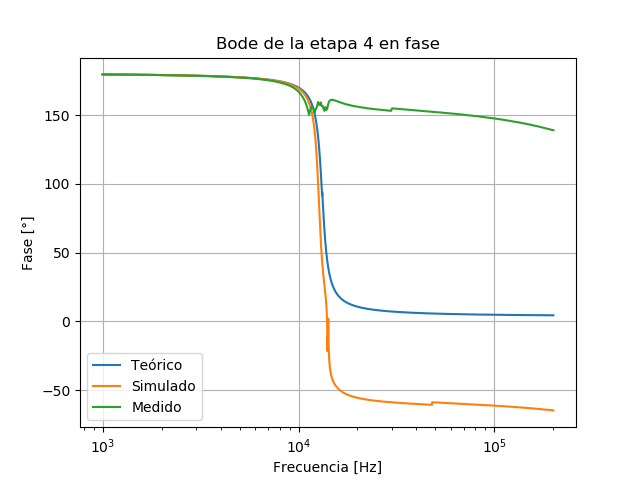
\includegraphics[width=\textwidth]{Imagenes/Pha-4.png}
	\caption{Diagrama de Bode de la cuarta etápa en fase.}
	\label{fig:pha4}
\end{subfigure}
\centering
\begin{subfigure}{.49\textwidth}
\centering
	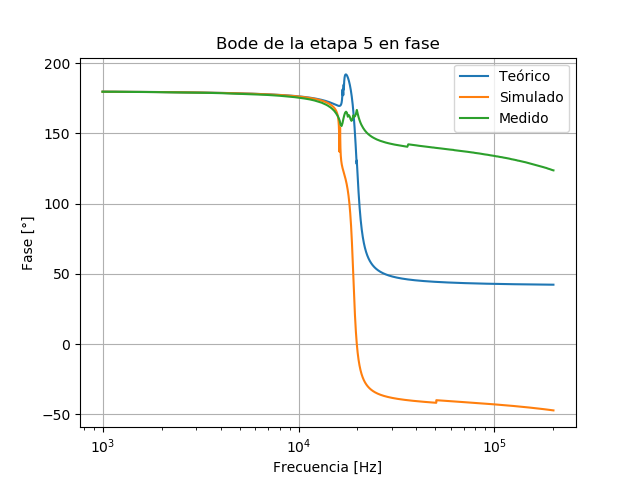
\includegraphics[width=\textwidth]{Imagenes/Pha-5.png}
	\caption{Diagrama de Bode de la quinta etápa en fase.}
	\label{fig:pha5}
\end{subfigure}
\centering
\begin{subfigure}{.49\textwidth}
\centering
	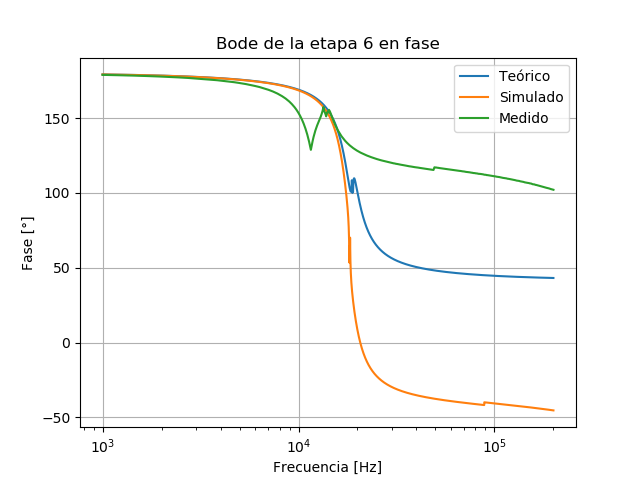
\includegraphics[width=\textwidth]{Imagenes/Pha-6.png}
	\caption{Diagrama de Bode de la sexta etápa en fase.}
	\label{fig:pha6}
\end{subfigure}
\caption{Comparación de los Bodes de las etapas en fase.}
\label{fig:bode-pha}
\end{figure}

Finalmente, se optó por medir la ganancia de tensión del sistema y contrastarla con la plantilla deseada, de esta forma se puede corroborar con mayor facilidad el logro del objetivo deseado.
\begin{figure}[H]
\centering
\begin{subfigure}{.7\textwidth}
\centering
	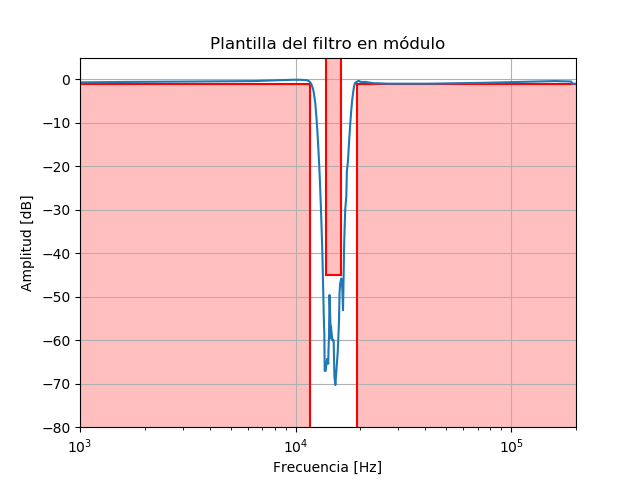
\includegraphics[width=\textwidth]{Imagenes/Mod-Plantilla-1.png}
	\caption{Totalidad del filtro medido.}
	\label{fig:filtro1}
\end{subfigure}
\centering
\begin{subfigure}{.7\textwidth}
\centering
	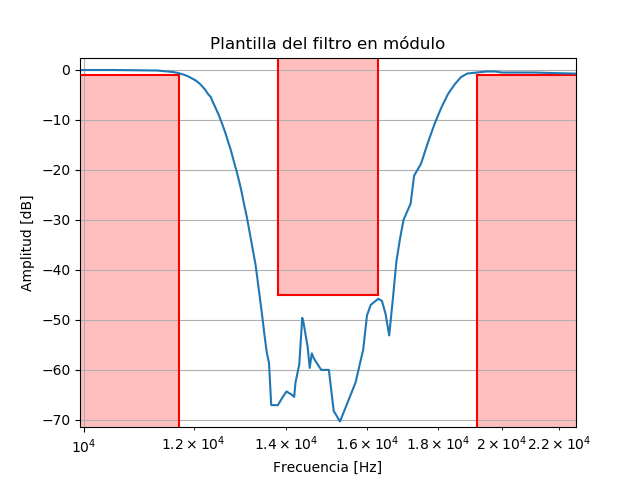
\includegraphics[width=\textwidth]{Imagenes/Mod-Plantilla-2.png}
	\caption{Banda atenuante.}
	\label{fig:filtro2}
\end{subfigure}
\caption{Medición del filtro y su respectiva plantilla.}
\label{fig:filtro}
\end{figure}

\subsection{Rango dinámico}
El rango dinámico se define como la razón entre el máximo y el mínimo valor que puede tomar el observable de interés. Para el caso en cuestión queda definido de la siguiente manera:
\begin{equation}
	R_d = 20 \log_{10} \left( \frac{V_{in_{max}}}{V_{in_{min}}} \right)
\end{equation}

Para definir $V_{in_{min}}$ se tuvo en cuenta la tensión mínima que se puede distinguir respecto al piso de ruido, la cual es determinada como $V_{in_{min}} \approx 10 \ mV$. Luego, para el caso de $V_{in_{max}}$, se consideró la máxima tensión previa a la aparición de distorsiones o alinealidades del amplificador operacional, siendo el cross-over, slew-rate y saturación del mismo algunos de estos efectos. Tanto el cross-over como el slew-rate son aspectos de poco interés, dado que, como para este filtro se seleccionó el amplificador \href{http://www.ti.com/lit/ds/symlink/tl082.pdf}{LM833}, ya que posee un elevado slew-rate y, dada su etapa de salida, el efecto de cross-over no genera problemas. Es así que, dada los sobre picos existentes, se determinó que esta tensión máxima es de $2 \ V$, de esta forma se determina el rango dinámico:
\begin{equation}
	R_d = 20 log \left( \frac{V_{max}}{V_{min}} \right) = 46.02 \ dB 
\end{equation}

\subsection{Máxima carga}

\subsection{Ganancia de lazo}
Se simuló la ganancia de lazo del sistema. Ya que para cada etapa, el resultado obtenído es para cada caso el mismo, presentando pequeñas diferencias propias de los componentes seleccionados. Esto se debe a que todas las empleadas son celdas universales del tipo Fleischer-Tow, por lo que es epserable dicho resultado. Es así se optó por presentar la simulación de la primer etápa y generalizar para las demás.
\begin{figure}[H]
\centering
	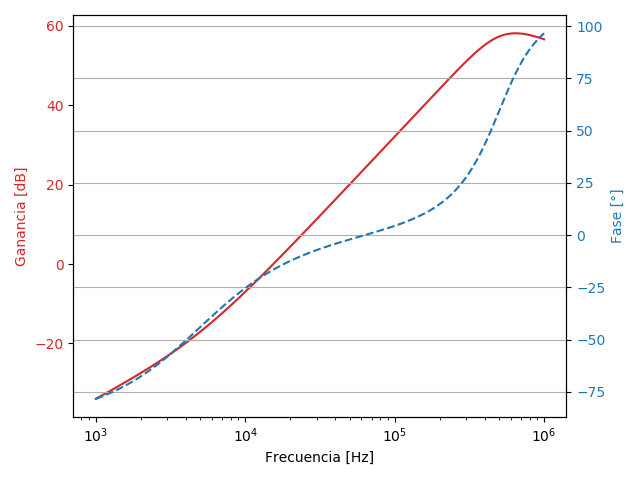
\includegraphics[width=0.5\textwidth]{Imagenes/GananciaDeLazo.png}
	\caption{Ganancia de lazo de cada etapa.}
\label{fig:lazo}
\end{figure}

Se observa de este que, dado que la frecuencia nunca alcanza los $180^o$ de desfazaje, el sistema cumple con la condición de Barkhausen demostrando estabilidad.


\end{document}